\documentclass[12pt,a4paper,utf8x,oneside]{report}
\usepackage [english]{babel}
% Pour pouvoir utiliser 
\usepackage{ucs}
\usepackage[utf8x]{inputenc}

\usepackage{pifont}
\newcommand{\tick}{\ding{51}} % to write ticks
\newcommand{\badtick}{\ding{55}} % to write cross

\usepackage[pdftex]{graphicx} % to include pictures
\usepackage{pdfpages} % to include PDF pages as pictures (1st and last page)

\usepackage{url} % Pour avoir de belles url
\usepackage[top=2.5cm, bottom=2.5cm, left=2.5cm, right=2.5cm]{geometry}


\usepackage{wrapfig}
\usepackage{subfig}

\usepackage{color}
\usepackage{xcolor}



% Pour mettre du code source
\usepackage {listings}
% Pour pouvoir passer en paysage
%\usepackage{lscape}

\usepackage{caption}
\DeclareCaptionFont{white}{\color{white}}
\DeclareCaptionFormat{listing}{\colorbox{gray}{\parbox{\textwidth}{#1#2#3}}}
\captionsetup[lstlisting]{format=listing,labelfont=white,textfont=white}

\lstdefinelanguage{JavaScript}{
     keywords={attributes, class, classend, do, empty, endif, endwhile, fail, function, functionend, if, implements, in, inherit, inout, not, of, operations, out, return, set, then, types, while, use},
     keywordstyle=\color{blue}\bfseries,
     ndkeywords={},
     ndkeywordstyle=\color{yellow}\bfseries,
     identifierstyle=\color{black},
     sensitive=false,
     comment=[l]{//},
     commentstyle=\color{green}\ttfamily,
     stringstyle=\color{red}\ttfamily
  }

  \usepackage{courier}
 \lstset{
         basicstyle=\footnotesize\ttfamily, % Standardschrift
         %numbers=left,               % Ort der Zeilennummern
         numberstyle=\tiny,          % Stil der Zeilennummern
         %stepnumber=2,               % Abstand zwischen den Zeilennummern
         numbersep=5pt,              % Abstand der Nummern zum Text
         tabsize=2,                  % Groesse von Tabs
         extendedchars=true,         %
         breaklines=true,            % Zeilen werden Umgebrochen
         keywordstyle=\color{red},
    		frame=b,      	
    	 identifierstyle=\ttfamily,   
		 keywordstyle=\color[rgb]{0,0,1},
         commentstyle=\color[rgb]{0.133,0.545,0.133},
         stringstyle=\color[rgb]{0.627,0.126,0.941},
         %stringstyle=\color{white}\ttfamily, % Farbe der String
         showspaces=false,           % Leerzeichen anzeigen ?
         showtabs=false,             % Tabs anzeigen ?
         xleftmargin=17pt,
         framexleftmargin=17pt,
         framexrightmargin=5pt,
         framexbottommargin=4pt,
         %backgroundcolor=\color{lightgray},
         showstringspaces=false      % Leerzeichen in Strings anzeigen ?        
 }
 
 \lstloadlanguages{XML, HTML,Java,PHP,SQL,JavaScript,bash,Ant}


% Pour pouvoir faire plusieurs colonnes
%\usepackage {multicol}
% POur crééer un index
\usepackage{makeidx}
\makeindex

% Pour les entetes de page
%\usepackage{fancyhdr} % Header and footnotes
%\pagestyle{fancy}
%\renewcommand{\chaptermark}[1]{\markboth{#1}{}}
%\renewcommand{\sectionmark}[1]{\markright{\thesection\ #1}}
%\fancyhf{} \fancyhead[LE,RO]{\bfseries\thepage}
%\fancyhead[LO]{\bfseries\rightmark}
%\fancyhead[RE]{\bfseries\leftmark}
%\renewcommand{\headrulewidth}{0.5pt}
%\addtolength{\headheight}{0.5pt}
%\addtolength{\headwidth}{100pt }
%\renewcommand{\footrulewidth}{0pt}

% Pour l'interligne de 1.5
\usepackage {setspace}
% Pour les marges de la page
%\geometry{a4paper, top=2.5cm, bottom=3.5cm, left=1.5cm, right=1.5cm, marginparwidth=1.2cm}

%for more little space between list items use : \begin{itemize*} instead of \begin{itemize} for compact lists
\usepackage{mdwlist}

\parskip=7pt %% distance entre § (paragraphe)
%\sloppy %% respecter toujours la marge de droite 

% Pour les pénalités :
%\interfootnotelinepenalty=150 %note de bas de page
%\widowpenalty=150 %% veuves et orphelines
%\clubpenalty=150 

%Pour la longueur de l'indentation des paragraphes
%\setlength{\parindent}{15mm}

\usepackage[toc,page]{appendix}
\usepackage{hyperref}
%%%% debut macro pour enlever le nom chapitre %%%%
%\makeatletter
%\def\@makechapterhead#1{%
%  \vspace*{50\p@}%
%  {\parindent \z@ \raggedright \normalfont
%    \interlinepenalty\@M
%    \ifnum \c@secnumdepth >\m@ne
%        \Huge\bfseries \thechapter\quad
%    \fi
%    \Huge \bfseries #1\par\nobreak
%    \vskip 40\p@
%  }}
%
%\def\@makeschapterhead#1{%
%  \vspace*{50\p@}%
%  {\parindent \z@ \raggedright
%    \normalfont
%    \interlinepenalty\@M
%    \Huge \bfseries  #1\par\nobreak
%    \vskip 40\p@
%  }}
%\makeatother
%%%% fin macro %%%%

%Couverture 
% Le plus simple est d'importer un pdf s'il y a une couverture type a respecter
%
\includepdf[pages=1,noautoscale=false]{premiere_page.pdf} 


\begin{document}

\includepdf[pages=1,noautoscale=false]{Couv_rapport_Marc.pdf}
%\maketitle

\chapter*{Acknowledgements}
First I would like to thank Mr. TAEI Payman, Director of Operations and President of
Hindsite Interactive for allowing me to integrate this structure and have this unique
opportunity to realize my final degree project in the United States.
In particular I would like to thank Mr. TAEI for the confidence he granted to me to
lead the different projects I was affected to by considering me as an employee.
As my tutor I want to thank him for proposing me interesting, diversified and original
projects and tasks from a technical point of view. I especially enjoyed the autonomy
and responsibilities he entrusted me. But also follow-up, availability, advice and
criticism that enabled me to make progress and improve at the technical point of
view as well as methodological.
As well thank you to Mr. KHERADMAND Shayan, responsible of design who was
one of my co-worker and contact for all questions regarding the design. He was
always available and relevant in his answers.

I also would like to thank Mr. WEINZAPFEEL Pierre, ex-intern at Hindsite extending his
experience in the company for other six-months as a Web Developer. He was my
main co-worker and a precious help to understand the architecture and existing
code. Our mutual help allowed us to achieve a working project and a quick
progression of tasks.

Finally I thank all other employees of Hindsite at a distance or not for their patience
and help when needed.
%\clearpage

\tableofcontents
\listoffigures
\listoftables
\clearpage

% Pour avoir un interligne de 1,5
\begin{onehalfspace}

\chapter{Introduction}

During my last year of studies at the University of Technology of Belfort-
Montbeliard (UTBM) in Computer Science Engineering, I acquired the
theoretical fundamentals in computer engineering, more particularly in
Software and Knowledge Engineering. In order to achieve my master in
engineering degree, my curriculum requires a 24-weeks final degree project to
apply and develop my skills in a professional activity.

I have chosen to apply to do this internship at Hindsite Interactive in order to
go into details in the web development and multimedia fields of study, an area
in expansion that interests me more particularly. In addition I wanted to do this
project in a foreign country to continue my international experience initiated
with my ST40 (technical internship) in Basel, Switzerland. The project that
Hindsite offered me was ambitious and required the mastery of a range of
different technologies.

Hindsite Interactive is a small business specialized in multimedia, web
development, web design and website hosting. The main services proposed
are designing, web site creation and an online tool that can be compared to a
Content Management System (CMS) called Easy Web Content (EWC). This
tool allows customers to create a new website, edit an existing one and
manage their sites.

My internship as a junior web developer has for main task to create new add-
ons for EWC and to develop a manager to enable clients to create, customize,
edit and populate these add-ons. An add-on is defined as an interactive
dynamic module that can be embedded in their website by clients. The goal is
to realize a common structure for all add-ons to reduce development time for
further add-ons.

After a presentation of the company and the Easy Web Content site, I will
describe the organization of the internship and finally detail the achieved work.

\clearpage


%samples chapter
%\chapter{Le titre du chapitre}

\section{Le titre de la section qui va bien}

\subsection{Titre de la sous section}

Exemple de code .
\lstset{language=HTML}
\begin{lstlisting}[label=some-css,caption=Some Html]
<style>
.header {
	background:#333;
	height:123px;

}
</style>

\end{lstlisting}
\lstset{language=PHP}
\begin{lstlisting}[label=some-php,caption=Some Php]
<?php
public class maClasse{
	public maFonction()
	{
		$maVar = new String("hello world");	
	}
}
?>

\end{lstlisting}
%$
\lstset{language=JavaScript}
\begin{lstlisting}[label=some-js,caption=Some JavaScript]

var mavar = new String('polop');
alert("hello world");
return false;

\end{lstlisting}

\lstset{language=SQL}
\begin{lstlisting}[label=some-sql,caption=Some SQL]

SELECT * FROM page WHERE id='1';

\end{lstlisting}

%-- Note de bas de page sur les stades
\protect\footnote{Par exemple, on peut faire un pied de page :
\begin{itemize}
\item avec une liste à puces ;
\item avec une liste à puces ;
\item avec une liste à puces.
\end{itemize}
}
%-- Fin Note de bas de page sur les stades

Ici du texte et du blabla, ce que l'on veut dire et écrire. A remplacer. Ici du texte et du blabla, ce que l'on veut dire et écrire. A remplacer. Ici du texte et du blabla, ce que l'on veut dire et écrire. A remplacer. Ici du texte et du blabla, ce que l'on veut dire et écrire. A remplacer. Ici du texte et du blabla, ce que l'on veut dire et écrire. A remplacer. Ici du texte et du blabla, ce que l'on veut dire et écrire. A remplacer.

\begin{itemize}
\item avec une liste à puces ;
\item avec une liste à puces ;
\item avec une liste à puces.
\end{itemize}

Ici du texte et du blabla, ce que l'on veut dire et écrire. A remplacer. Ici du texte et du blabla, ce que l'on veut dire et écrire. A remplacer. Ici du texte et du blabla, ce que l'on veut dire et écrire. A remplacer. Ici du texte et du blabla, ce que l'on veut dire et écrire. A remplacer. Ici du texte et du blabla, ce que l'on veut dire et écrire. A remplacer. Ici du texte et du blabla, ce que l'on veut dire et écrire. A remplacer.

\subsubsection{Titre de la sous sous section}

Ici du texte et du blabla, ce que l'on veut dire et écrire. A remplacer. Ici du texte et du blabla, ce que l'on veut dire et écrire. A remplacer. Ici du texte et du blabla, ce que l'on veut dire et écrire. A remplacer. Ici du texte et du blabla, ce que l'on veut dire et écrire. A remplacer. Ici du texte et du blabla, ce que l'on veut dire et écrire. A remplacer. Ici du texte et du blabla, ce que l'on veut dire et écrire. A remplacer.

%exemple d'image
\begin{figure}[!ht]
\centering
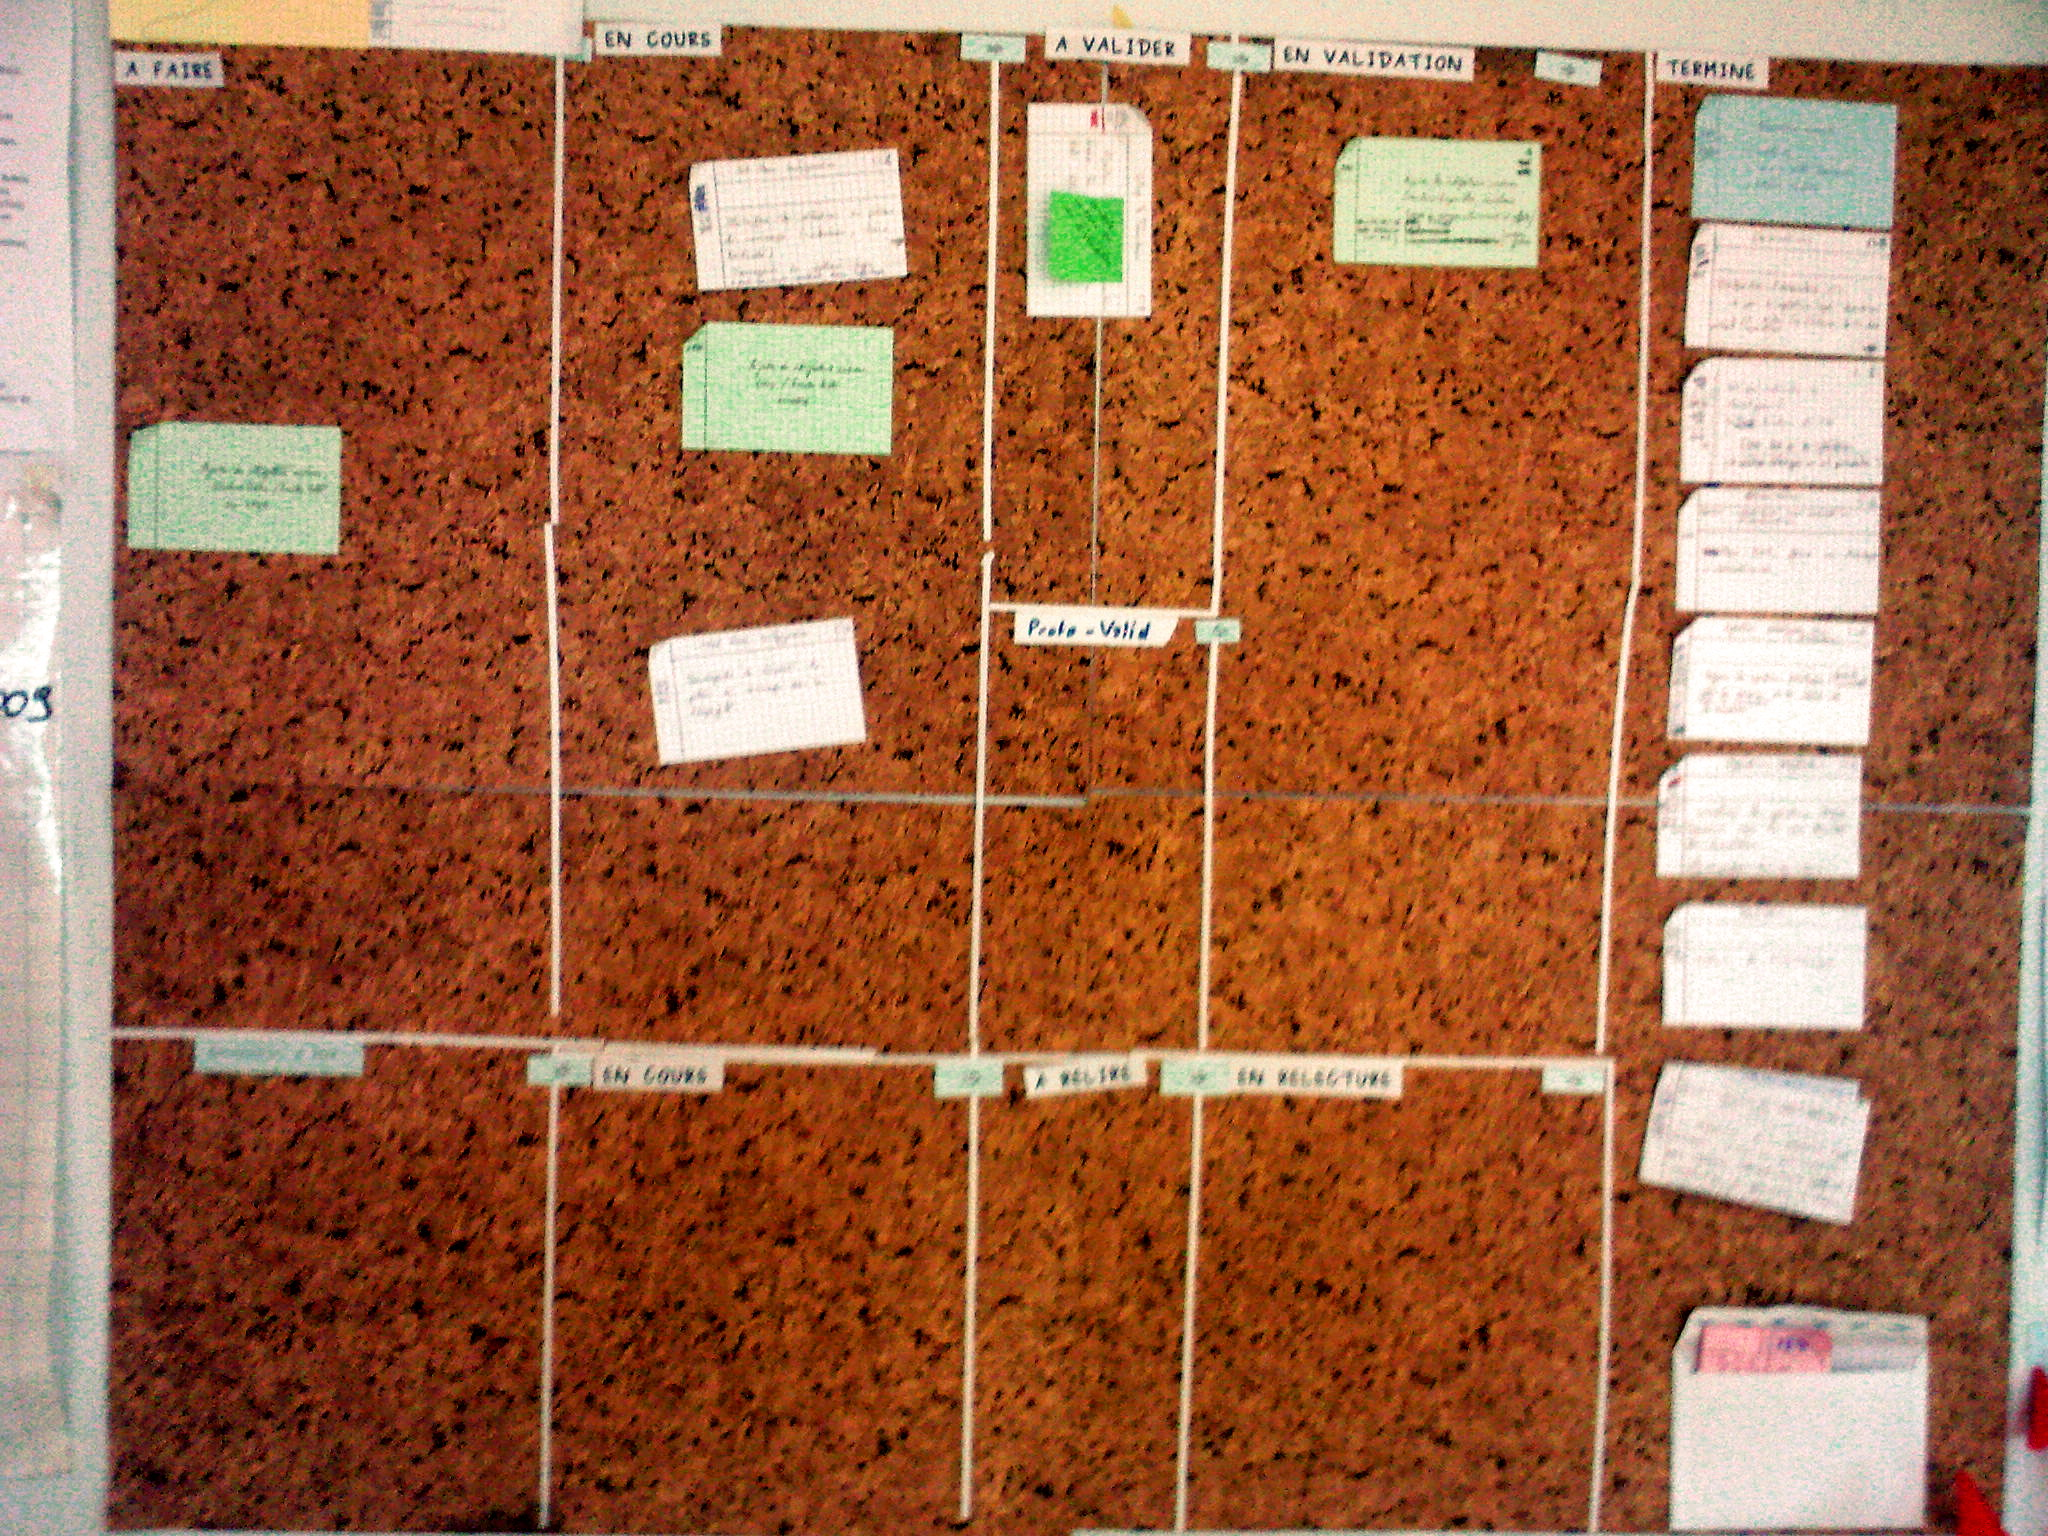
\includegraphics[width=.55\textwidth]{img/SP_A0183.jpg}
\caption{Image sample}
\label{figure:sampe}
\end{figure}

Ici du texte et du blabla, ce que l'on veut dire et écrire. A remplacer. Ici du texte et du blabla, ce que l'on veut dire et écrire. A remplacer. Ici du texte et du blabla, ce que l'on veut dire et écrire. A remplacer. Ici du texte et du blabla, ce que l'on veut dire et écrire. A remplacer. Ici du texte et du blabla, ce que l'on veut dire et écrire. A remplacer. Ici du texte et du blabla, ce que l'on veut dire et écrire. A remplacer.

\subsubsection{Titre de la sous sous section}

Exemple de tableau
\begin{table}[!ht]
	\caption{\label{tableau:evolPratXP}Evolution des pratiques XP au cours du stage}
	\begin{tabular}{|l|c|c|}
		\hline
		Pratique & Début du stage & Fin du stage\\
		\hline
		Pair programming & \tick & \tick \\
		Itération & 2 semaines & 1 semaine \\
		Intégration continue & \tick & \tick \\
		Niko Niko & \tick & \badtick \\
		Lecture & \tick & \badtick \\
		Point perso & hebdomadaire & nouvelles experimentations\\
		Pomodoro & \badtick & \tick \\
		Test driven development & \tick & \tick \\
		``Done done'' & théorique & adopté et normalisé\\
		``No Bugs'' & imprécis & engagement \\
		Slack Time & \badtick & adopté et normalisé\\
		Rétrospective & 1 à 2h le lundi matin & Timeboxée et juste après la livraison\\
		Point technique & assez réguliers & moins nombreux\\
		Veilleur & \tick & Robin cumule son rôle\\
		Batman/Robin & \badtick & \tick \\
		\hline
	\end{tabular}
\end{table}

\subsection{Conclusion}

Ici du texte et du blabla, ce que l'on veut dire et écrire. A remplacer. Ici du texte et du blabla, ce que l'on veut dire et écrire. A remplacer. Ici du texte et du blabla, ce que l'on veut dire et écrire. A remplacer. Ici du texte et du blabla, ce que l'on veut dire et écrire. A remplacer. Ici du texte et du blabla, ce que l'on veut dire et écrire. A remplacer. Ici du texte et du blabla, ce que l'on veut dire et écrire. A remplacer.

Ici du texte et du blabla, ce que l'on veut dire et écrire. A remplacer. Ici du texte et du blabla, ce que l'on veut dire et écrire. A remplacer. Ici du texte et du blabla, ce que l'on veut dire et écrire. A remplacer. Ici du texte et du blabla, ce que l'on veut dire et écrire. A remplacer. Ici du texte et du blabla, ce que l'on veut dire et écrire. A remplacer. Ici du texte et du blabla, ce que l'on veut dire et écrire. A remplacer.

\subsection{Titre de la sous section}

Ici du texte et du blabla, ce que l'on veut dire et écrire. A remplacer. Ici du texte et du blabla, ce que l'on veut dire et écrire. On peut faire une citation \cite{Motclef1}.
A remplacer. Ici du texte et du blabla, ce que l'on veut dire et écrire. A remplacer. Ici du texte et du blabla, ce que l'on veut dire et écrire. A remplacer. Ici du texte et du blabla, ce que l'on veut dire et écrire. A remplacer. Ici du texte et du blabla, ce que l'on veut dire et écrire. A remplacer.

Ici du texte et du blabla, ce que l'on veut dire et écrire. A remplacer. Ici du texte et du blabla, ce que l'on veut dire et écrire. A remplacer.
Ici du texte et du blabla, ce que l'on veut dire et écrire. A remplacer. Ici du texte et du blabla, ce que l'on veut dire et écrire. A remplacer. Ici du texte et du blabla, ce que l'on veut dire et écrire. A remplacer. Ici du texte et du blabla, ce que l'on veut dire et écrire. A remplacer.

\subsection{Titre de la sous section}

Ici du texte et du blabla, ce que l'on veut dire et écrire. A remplacer. Ici du texte et du blabla, ce que l'on veut dire et écrire. On peut faire une citation \cite{Motclef1}.
A remplacer. Ici du texte et du blabla, ce que l'on veut dire et écrire. A remplacer. Ici du texte et du blabla, ce que l'on veut dire et écrire. A remplacer. Ici du texte et du blabla, ce que l'on veut dire et écrire. A remplacer. Ici du texte et du blabla, ce que l'on veut dire et écrire. A remplacer.

Ici du texte et du blabla, ce que l'on veut dire et écrire. A remplacer. Ici du texte et du blabla, ce que l'on veut dire et écrire. A remplacer.
Ici du texte et du blabla, ce que l'on veut dire et écrire. A remplacer. Ici du texte et du blabla, ce que l'on veut dire et écrire. A remplacer. Ici du texte et du blabla, ce que l'on veut dire et écrire. A remplacer. Ici du texte et du blabla, ce que l'on veut dire et écrire. A remplacer.

\clearpage


%productivity tools
%projects

\chapter{Company presentation}

\section{Presentation}

Hindsite Interactive is a small-size enterprise located in Frederick, Maryland at
approximately 45 minutes to the large city of Washington DC. Hindsite owns a
subsidiary Webnet Hosting based in Rockville, at the periphery of Washington
DC. Both Frederick and Rockville are under the area of effect of the capital
city whose total agglomeration counts more than 5 billion inhabitants.

\textbf{Headquarter} \\
Hindsite Interactive Inc.\\
241 East 4th Street\\
Frederick, Maryland 21701 USA\\

\subsection*{Short History}

Hindsite Interactive is a young company founded in 2000 by the actual
President of Operation, Mr. Payman Taei. Everything started from the corner
of a small apartment, \$170 and a vintage Pentium processor and is now a
business with two divisions. As written on Hindsite Interactive website: his main goal is not to form a conglomerate corporation but to provide a quality service and to maintain a
strong relationship with each of his client.

\section{Organizational Unit}

Hindsite is a very small company, it counts in total between 10 and 12
employees and they are not all working in the same place. The following diagram is a representation of the organization unit at Hindsite
Interactive.

\begin{figure}[ht]
\centering
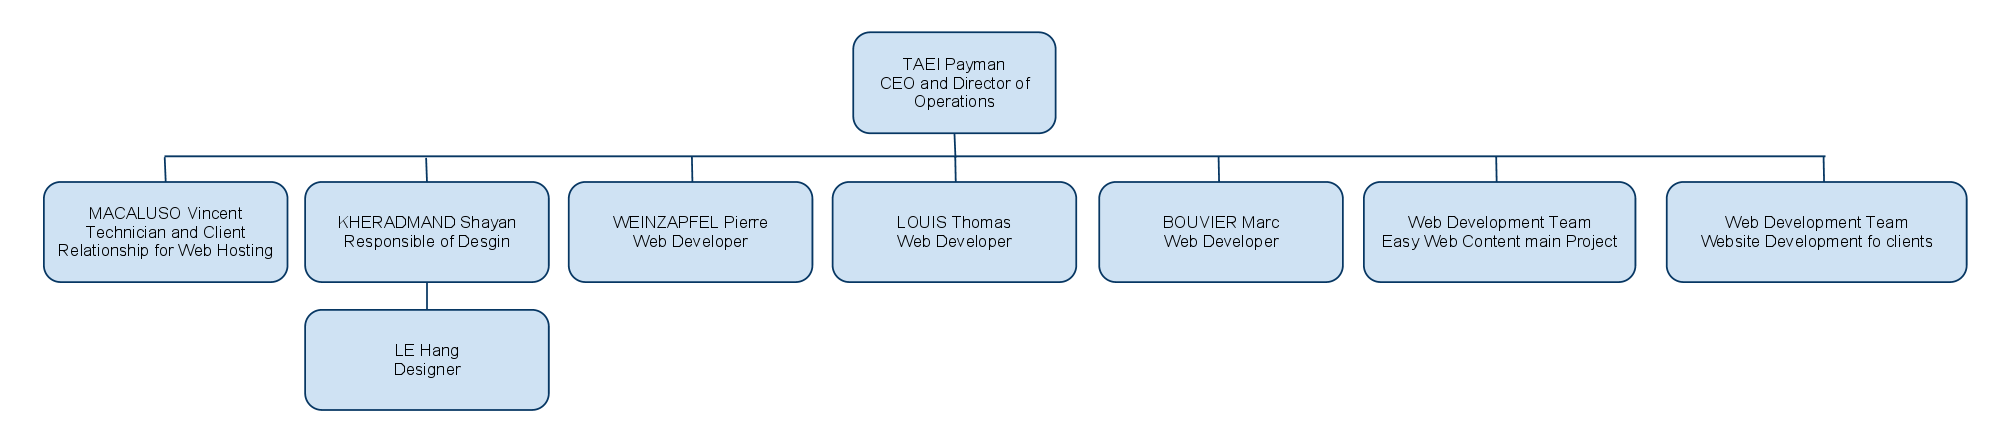
\includegraphics[width=\textwidth]{img/hindsite_organigramme.png}
\caption{Hindsite Interactive Hierarchy}
\label{figure:organigramme}
\end{figure}

My role at Hindsite Interactive takes place in the development team, as a
junior web developer. My hierarchic superior is Mr. Payman Taei, who assign
my tasks most of the time. But I am also working closely from the designer Mr.
Shayan Kheradmand to take over the design phase with the development one.
During all my internship I was working in collaboration with Mr. Pierre
Weinzapfel, web-developer and ex UTBM student.
Finally I have always been in touch with other developers at Hindsite who are
working from a different geographic place.

\section{Company activities}

Hindsite Interactive proposes different services though its different labels.
Around the Hindsite Interactive name are gathered:
\begin{itemize}
\item The web design and web development
\item Graphic design and interfaces
\item 3D modeling
\item Animation and interactivity
\end{itemize}
The website development is diversified but essentially centered on the CMS,
e-commerce and dynamic applications.

\subsection*{Webnet Hosting}

This subsidiary from Hindsite Interactive takes care of the management and
hosting of websites. In addition, the company offers a large number of
services that are a success with not less than a thousand websites hosted.

Overview of the main services and characteristics:
\begin{itemize}
\item Easy Web Content: the website editor
\item A CMS: Site Studio Design that proposes 600 templates
\item Urchin for analysis and statistics
\item Word Press for the realization of forums, blogs, pools etc.
\item CPanel, for site configuration and management
\item Full backup every night
\end{itemize}
Since his creation Hindsite proposes solutions in term of design and animation
that use the newest technologies and therefore has a recognized know-how in
his field of competence.
A proof is Hinsite’s website entirely realized in Flash and animated. This site is
a portfolio itself of the company competences.
The company received awards for his website and the quality of work from
“PC World”, “Best of the Web”, “Perfectory Award” and the “Golden Web
Award” by The International Association of Web Masters and Designers.

\section{Clients}

Even though Hindsite is still a young company, it owns already an extended contact
list. Here are some example of customer and projects:


\begin{description}
  \item[ABC News]A division of the famous television channel ABC, one of the
four top networks in the US. ABC News is a national news channel. Hindsite
realized a module for the website to cover the last presidential campaign.
  \item[Avalere]A leading advisory company focused on healthcare business
strategy and public policy. Our company realizes different projects for
Avalere’s customers.
  \item[Noland Aviation] an aircraft sales and acquisition company. Hindsite
Interactive entirely designed and developed the website and Flash animations.
  \item[Sentara College of Health Sciences] a university located in Virginia. It
belongs to the Sentara Health System organization that counts a hundred of
sites. Hindsite designed a website with a full CMS.
  \item[Bay Area Biomedical Consultants Network] provides
networking and educational opportunities for consultants in the San Francisco
life sciences community. Another example of a website developed by Hindsite
Interactive and in which I participated in the development.
  \item[Sencore] a manufacturer and retailer of high precision video and hifi transcoders.
\ldots
\end{description}


Through these examples we see that clients come from various fields like
industry, services, consulting, education, health, Medias, etc.
This shows that Hindsite knows how to adapt to the specific needs of the
different clients.

\section{Services proposed}

\subsection{Complete website development}

Hindsite proposes its clients to create their websites from A to Z, including the
specification, the design, the development, eventually an administration
section and hosting on its server.

\subsection{Other design projects}

This can be a CD/DVD presentation, a logo, a Flash animation or banner, a
company presentation in a video format, advertisements, etc.

\subsection{Easy Web Content}
%easy web content image
\begin{figure}[!ht]
\centering

\includegraphics[width=.30\textwidth]{img/ewc.png}
\caption{Easy Web Content Logo}
\label{figure:ewc-logo}
\end{figure}

Easy Web Content is a solution that can be compared to a CMS (Content
Management System). This innovative web platform allows website owners to
update easily and maintain their websites.

The solution proposed is entirely online and doesn’t require any download and
installation. As a matter of fact, the system is modular and flexible.
It is important to highlight that the system does not require any knowledge in web
development and everything is done to facilitate usability. Most of the users are
novice.

Easy Web Content allows users to manage their web pages, edit content, manager
their FTP server but also to add dynamic content to their pages as a music player, a calendar etc. Major possibilities of the software.

\begin{itemize}
\item Edition of all pages and content
\item Creation of web pages
\item Addition of interactive, dynamic content in Flash and/or HTML (all add-ons)
\item Security of pages with a login/password access
\end{itemize}

\section{Company Analyze}

Hindsite Interactive has a strategic geographic position, indeed Frederick is
located inside an agglomeration with a worldwide influence in the eastern
megalopolis of the USA and its main city New York City. This area is the
economical heart of the country and counts more than 55 million inhabitants.

It’s also one of the most influent in the world in the economical, financial,
political or even cultural aspects. All this favorites businesses of all kind and
especially requires new technologies and information systems (IT). As a
matter of fact, Hindsite Interactive occupies a central position that allows it to
answer quickly and efficiently to the customer needs.

Closer to Frederick, Washington DC is the capital of the USA and therefore
hosts thousands of federal institutions, organizations, law firms, medias,
consulting companies etc. Moreover the Washington area comprises
worldwide companies headquarters and some of the most famous universities
(e.g. Georgetown).

Hindsite knew how to take advantage of this heterogeneity by offering different
services and have client in all sectors. This non-specialization offers Hindsite
the ability to continue growing during the economical crisis.
In order to comply with the Business Model of the company, the philosophy is
to develop the interdisciplinary of competences and a quick adaptation to the
new technologies to answer the best to the client expectations.

\clearpage
\chapter{Internship Organization}

\begin{table}[!ht]
	\caption{\label{tableau:agenda}Internship Agenda}
	\begin{tabular}{ | l | p{12cm} | }
		\hline
		 & Tasks\\
		\hline
		Week 1	&	Population of content for Sencore's website\\	\hline
		Week 2	&	Development of Sencore's Website. Read documentation of the different projects of Hindsite Interactive. Get comfortable with the main project Easy Web content.\\	\hline
		Week 3 to 4	&	Work on Easy Web Content's Image Editor. Issues fixes.\\	\hline
		Week 5 to 7	&	Work both on the Image Editor and the specifications of the new Easy Web Content's Site Builder. Implementation of Performance Improvement tools.\\	\hline
		Week 8 to 12	&	Brainstorming and resarches about the Site builder features. Study the conpetitors. MVC Framework development.\\	\hline
		Week 12 to 16	&	Application of web design on the tools of the Site builder. Database development, drag and drop. User registration. Database automated scripts.	\\	\hline
		Week 17	to 18&	Work on Site Builder's widget features. Implementation of Video player feature on Sencore project. Work on secured payment form on A2LA project. Begin to communicate with clients.\\	\hline
		Week 19	to 22 &	Work on a mailling form for the client Advanced Centrifugals coupled with a backend. Bug correction on Sencore and Sentara projects. Work on the Site Builder in parallel\\	\hline
		Week 23	&	Work on Pylon Project\\	\hline
		Week 24	&	\\	\hline
	\end{tabular}
\end{table}
\chapter{My Image Editor}

This application (cf. \ref{figure:ewc-image_editor} p.\pageref{figure:ewc-image_editor}) could be compared to a standard image editor like Photoshop or The Gimp. It offers lot of possibilities to edit images (rotation, styles, filters ...). This big advantage of My Image Editor is that it does not require any installation on your computer (only the Adobe flash player and a web browser are required). A second strenght is that it can be used standalone (\url{http://myimageeditor.moreedits.com/Editor/editor.php}) or integrated to the Easy Web Content platform.


\begin{figure}[!h]
\centering
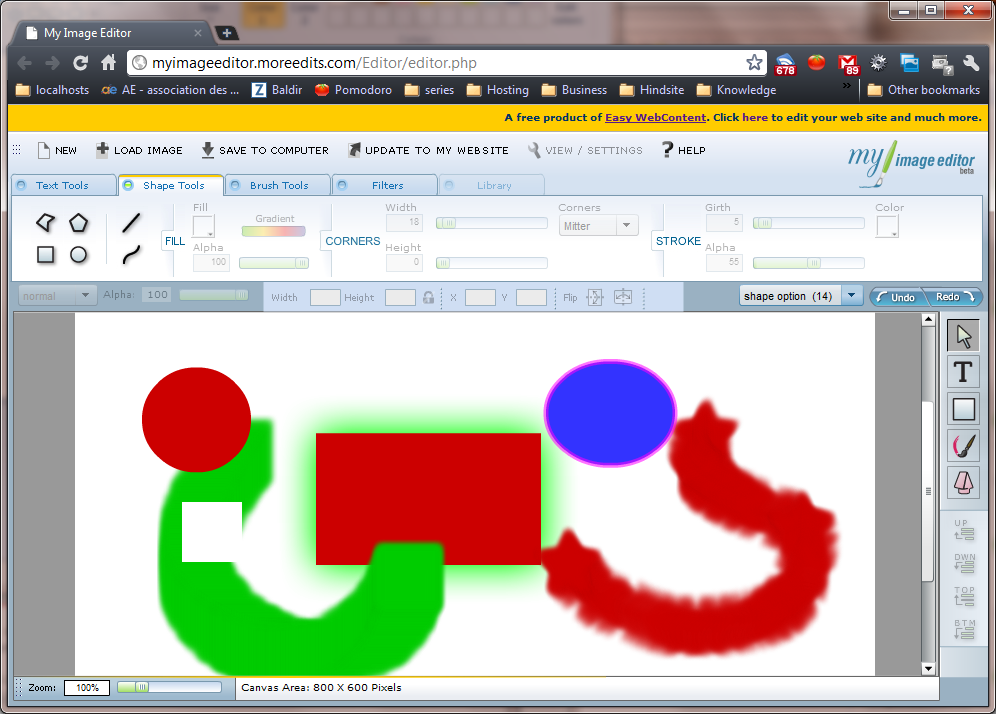
\includegraphics[width=.80\textwidth]{img/my_image_editor.png}
\caption{My Image Editor}
\label{figure:ewc-image_editor}
\end{figure}

I had first to "enter" head-first into the code written by the 3 previous interns. I was not very familiar with the Actionscript 3 programmation language but it is very similar to Java which I know better. One of the bigger difficulties was to deal with a main class file of more than 6000 lines of code. I could not refactor\footnote{Refactoring is a disciplined technique for restructuring an existing body of code, altering its internal structure without changing its external behavior (Martin Fowler \url{http://www.refactoring.com/)}} this piece of code because it would need too much time. 

I had to secure the swf file\footnote{file generated by Flash that can be embedded in a web page} by  using some URL rewrite technique and server side processing with PHP. Basically a PHP file with the .swf extension is used to import the file stream of the flash file. I added server directives to make .swf files interpreted as PHP scripts instead of directly downloaded. The PHP script require a session which is created by the script which want to embed the flash object. If the session is not found (which means that someone want to download the original .swf file by from its url it will return an error page instead of the file).

\lstset{language=PHP}
\begin{lstlisting}[label=swf-secure,caption=PHP script disguised into a swf file to avoid direct download]
	//retrieve the session
	session_start();
	//Test if the variable"flash" is directly access to prevent direct access by typing
	//the url of the swf file in the browser
	if(isset($_SESSION["flash"]))
	{
		$referrer = $_SERVER["HTTP_REFERER"];
		$referrer = parse_url($referrer);

		//Test if the domain are the same to prevent the access for others domains
		if($referrer["host"] != $_SESSION["flash"])
		{
			echo "Permission denied.";
			exit();
		}

	}
	else
	{
		echo "Permission denied.";
		exit();
	}
	//Destroy the session
	unset($_SESSION["flash"]);
	//Get the SWF if the test	
	header ("Cache-Control: no-cache, must-revalidate");
	header("Content-Type: application/x-shockwave-flash");
	readfile($_SERVER["DOCUMENT_ROOT"].'/Editor/01_Template.swf');
\end{lstlisting}
%$


I also had to add a preloader(cf. \ref{figure:ewc-image_preloader} p.\pageref{figure:ewc-image_preloader}) to the page embedding My Image Editor. The aim of this manipulation is to show a loading animation instead of a blank page while witing that the complete editor and its assets are fully loaded. In order to achieve this task the Image Editor had to communicate its status to the embedding page through a library called ExternalInterface. 

\begin{figure}[!h]
\centering
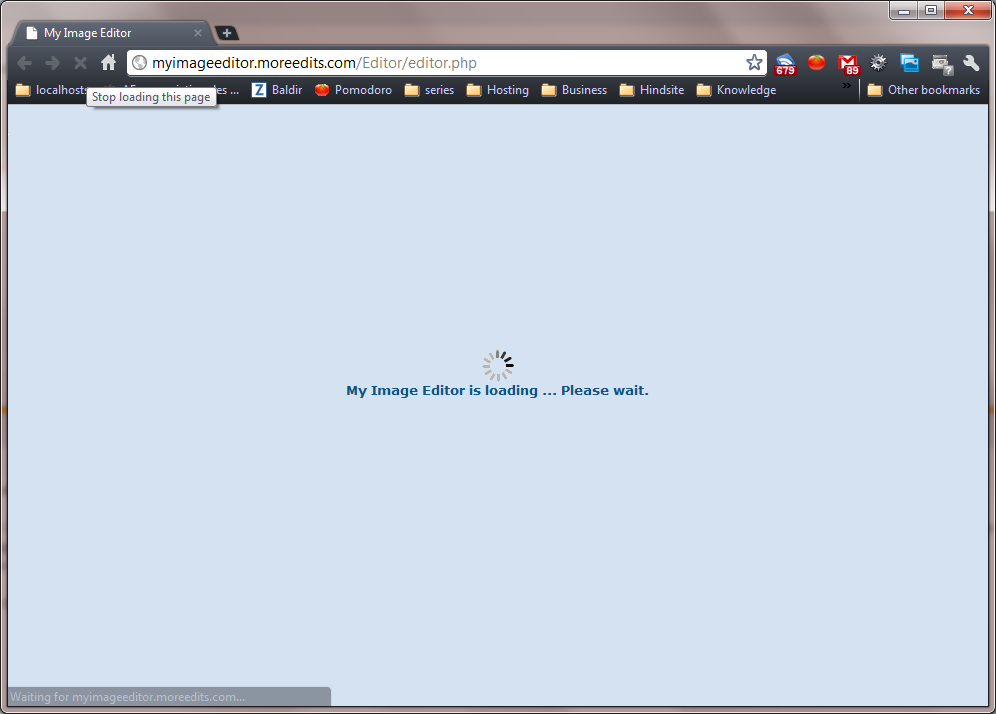
\includegraphics[width=.80\textwidth]{img/myimage_preloader.png}
\caption{My Image Editor preloader}
\label{figure:ewc-image_preloader}
\end{figure}

The other tasks were more flash related. Most of them were just little bug fixes such as brush issues, internal preloader, link to page, etc ...

After I worked enough on My Image Editor I continue to work on this project in parallel with the main project.
\chapter{Easy Web Content Site builder.}

The Easy Web Content Site Builder, also called EWS, is the main project we are working. This project intends to complete the existing Easy Web Content service by enabling the user to create a new website from scratch.
%descriptopn of EWS
Basically The site builder will make extensive usage of ajax. The main directions of the project are
\begin{itemize}
\item Be the most simple in terms of user experience
\item Propose simple to create but adapted styles and easy to customise
\item Do not have the drawbacks of the competitors
\item Have the advantages of the competitors
\item Be scalable
\item Be secure
\item Target users : 2/3 of them have no HTML/CSS knowledge
\end{itemize}
%show a sample of the concurrence

So the first step into the project was to brainstorm about the feasibility of the software. We did several research of what was already existing in the market. Writing dows the strengths and weaknesses of the most famous site builders. At the same time we specified the structure of the information system which would allow the site builder to be scalable, and modular. We try to figure what was the best choices between architecture and programming languages. After a week we decided to adopt PHP MySQL and Javascript instead of J2EE , GWT. The developers into the team are more familiar with these technologies. So we designed a relational model for the MySQL database that matched our first expectations in term of page creation and page organisation.
%several illustrations of the models evolution

\begin{figure}[!ht]
\centering
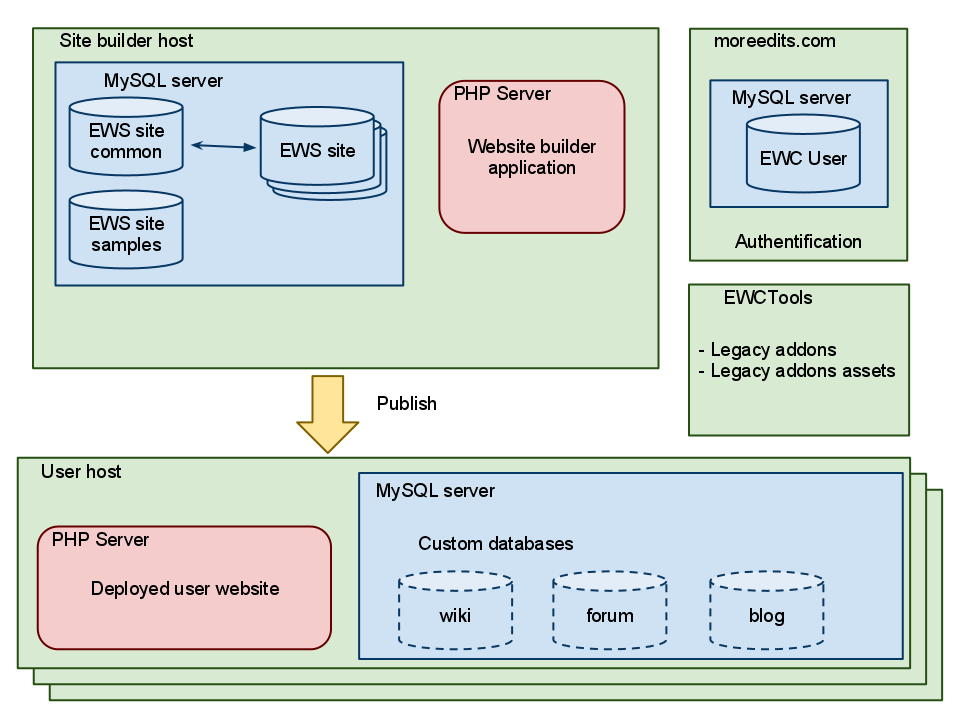
\includegraphics[width=.55\textwidth]{img/ews_archi_before.png}
\caption{Basic EWS architecture }
\label{figure:ews_archi_after}
\end{figure}


\begin{figure}[!ht]
\centering
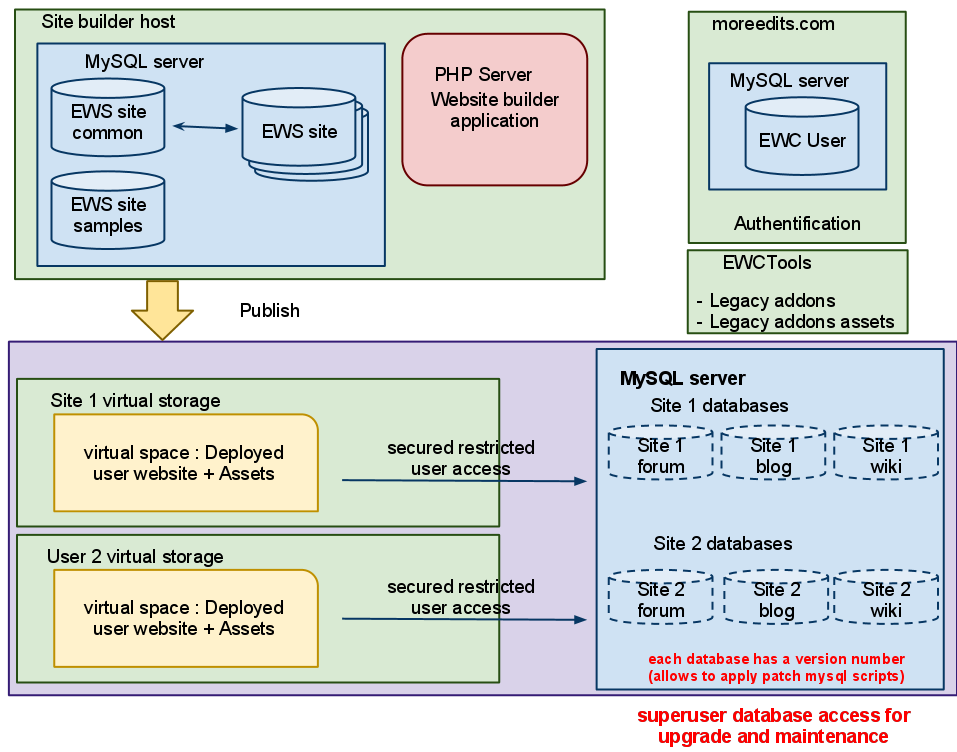
\includegraphics[width=.55\textwidth]{img/ews_archi_after.png}
\caption{EWS architecture rethought for cloud environment}
\label{figure:ews_archi_after}
\end{figure}

To allow scalability, security and future cloud architecture, we decided to split the application into several databases inside the same MySQL server. Inside the same MySQL server the databases can communicate easily with each other. So it allows to decouple these databases.
\begin{itemize}
\item a database to store common data (data shared through the application)
\item a database to manage users and sites
\item one database per site 
\end{itemize}
To allow better security, at the creation of a new site database the system creates a specific MySQL user for this database which have specific permissions only on that database. It can access common database data thru VIEWS.
% databases architecture illustration
After several meetings we decided to adopt a system that stores the informations of each pages created by the editor into a database. To allow less process time, the user will be able to publish his pages, which will result in the system creating plain php files containing all the information of the page.

\section{Framework}

To facilitate the development and maintainability of the application, we had to code using a Model View Controller pattern. The first thing that came to mind to adopt this pattern was to use a Php Framework. Many of them exist on the internet, for example Zend, Symphony, CakePhp, ... After looking at some of them, especially Zend, we figured out that using such a Framework would mean learning it. And it could be weeks before we were comfortable with it, let alone the fact that every six month new interns would come and would probably have to learn it too. The best solution for us considering the deadline we had on the project was to create our own MVC Framework. It took us less than a week to build the core features of this framework. Building our own framework has some advantages:
\begin{itemize}
\item In a learning point of view, it is very interesting as it would help us understand some useful mechanism of Php
\item We would have total control over it and would be able to add features as we need them.
\end{itemize}

The way our framework works is pretty simple. It redirect all request to one single entry point (index.php). This entry point would then call the appropriate controller and action. The controller then requests the database given the model we need and then call the appropriate view. This separates easily all 3 parts of the MVC pattern.
Also, the framework is object-based: 
\begin{itemize}
\item Each Controller is a Php class that inherits the core controller class. It contains all the functionalities needed to handle a page request, to redirect a page, to get the data sent by the user, ...
\item Each Model is a Php class that inherits the core model class. It contains all the functionalities to access the database and request it.
\item Each view is a phtml file in which we print the content of the request.
\end{itemize}
Developing an object-oriented application makes it way more scalable and reusable. It is the right way to develop a web application. During my 6 months at HindSite Interactive, I have worked on projects that had not been developed with object-oriented programming, and it was really hard to understand the code and be able to work efficiently with it. 

Later in the development of the application, we started adding features to the core of our framework. As an example, we created a special Controller, called AjaxController, that would be the type of controller to handle Ajax requests. Every other controller that would be called via Ajax would not process any treatment.
Another advantage of this framework is that the files are stored in different folders, so it is easier to localize the different elements. Most of the client projects I have worked on had all the files stored in one single folder, which can get really messy when this is a big project.
Here is the tree of the framework:
\begin{verbatim}
+---application
|   +---controllers
|   +---models
|   +---views
+---config
+---library
|   +---core
|   +---external
+---public
|   +---css
|   +---js
|   index.php
\end{verbatim}

\section{User Experience}

The main part of an application aimed at having people sign up for the services you provide is the user experience. If in the first few minutes of using the application the user feels lost or does not know how to perform the tasks he wants to, he is not going to sign up and will leave to the competitors. There are so many famous site builders in the Internet that we will surely not be the primary target of users. So when a user lands on our application, we need to keep him and have him sign up. So from the start of the development, we made a priority of providing the user with an easy interface, along with intuitive functionalities.
We had meetings once in a week to see which directions to take in terms of usability. Concerning the graphic user interface, the work was done by designers and we then had to convert their ideas to html and css code. The part that concerned us web developers was the intuitive functionalities. And in web language, this means programming in JavaScript / AJAX.

\subsection{JavaScript}

JavaScript is a client side programming language. It is interpreted by the user's web browser and runs on his computer, with no connection to the server whatsoever. When a web page is served to the user, JavaScript enables to extend the user experience. Some of the interesting functionalities of JavaScript are:
\begin{itemize}
\item Binding events to the mouse or keyboard of the user
\item Changing the way a page look
\item Handing the DOM (Document Object Model) which means Create, Read, Update or Delete the html content of the page.
\end{itemize}
One of the main user experience we wanted to provide to the user was enabling him to easily add or manage the content of its pages. A very powerful and intuitive way to achieve that goal is to have a Drag And Drop functionality. Basically what it does is bind an event to the user's mouse: when he clicks on an element, he can drag it and the element will follow the mouse position. When he releases the mouse, the element is placed according the the current mouse position. This is undoubtedly the most intuitive way to update the content of a page, as users are used to often drag and dropping in their Operating System. 
\\But usually, the easier and more intuitive it will be for the user, the more difficult it is going to be to implement it. Drag And Dropping does not avoid this rule. Hopefully, many tools (understand JavaScript libraries) exist on the web to perform this task. After testing all the most powerful tools existing, we choose to go with the one called Scriptaculous. By calling a simple method, Scriptaculous binds all the events needed to perform the drag and drop and adds callback functions for every of them. It is very powerful as it enabled you to run a script when beginning the drag and drop, when actually moving the element and when the element is dropped. 
\\But if JavaScript runs on the client's computer with no communication with the server, how can we save the result of the drag and drop so that when the user reloads the page, he will see what was intended ? The way to perform that is called Ajax.

\subsection{Ajax}

Ajax stands for Asynchronous JavaScript and XML. Nowadays, it is one of the most powerful tool to enable client/server communication without impacting the user. Let's take the example of the drag and drop. Before Ajax existed, to save the newly positioned element, we had to send a synchronous request to the server upon dropping the element. Basically that means the page the user was currently on would have to be refreshed in order for the user to see the changes. That could frustrate the user a lot as the page would have to be fully regenerated and resent to the user, and that process would take tenth of seconds, during which the user was not able to perform any task. Now, with Ajax, this does not have to happen this way anymore. Ajax permits requests to be sent to the server in an asynchronous way, which means that the page will not be refreshed and the user will not have to wait for the response to perform other actions. This is very powerful as it enables most of the scripting to be done server side and just called via Ajax, thus not preventing the user to perform other tasks. This gives a very good user experience as the user will not even notice that there was communication with the server.

\section{Web issues}

To understand the issues that arises when developing a web site or web application, let me first remind you how a user can access a web page.
\begin{itemize}
\item First, the client (the user's web browser) requests a web page located on a web server. The function of this web server is to deliver the requested web page to the client. This means delivery of an HTML document along with additional content, 
such as images, stylesheets and JavaScripts.
\item The client's web browser application then processes the content and displays it for the user.  
\end{itemize}

\begin{figure}[!l]
\centering
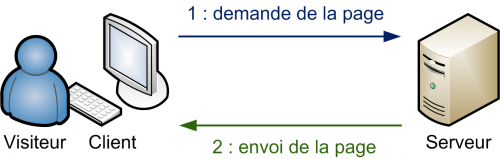
\includegraphics[width=.55\textwidth]{img/static.png}
\caption{Case of a static Html page}
\label{figure:static page}
\end{figure}
\begin{figure}[!r]
\centering
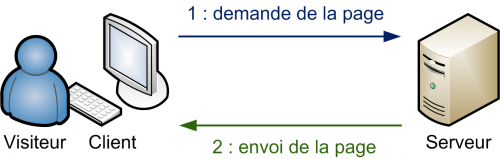
\includegraphics[width=.55\textwidth]{img/static.png}
\caption{Case of a dynamic page (for example a php page)}
\label{figure:dynamic page}
\end{figure}

While the server will always deliver the same content for the same requested page, two different users might see two different things on their computer. 
The reason is that there are more than one web browser software application existing, and while they try to make it look the same, the process behind the display and interpretation of the content is not. Set aside Html content, which is quite processed in the same way among every browsers, issues arises with interpretation of
JavaScript and Stylsheets (CSS). For example, Firefox will understand the CSS property moz-border-radius while Google Chrome and Internet Explorer will not. Also, Firefox will not understand the JavaScript Object window.event while Google Chrome and Internet Explorer will. There are dozens of example like these ones.
While you can develop the server side part of the application in one language and not worry about its ability to always deliver the same content, you can't afford to develop the client side application for only one browser. This would result in many internet users not to be able to see the content as intended.
\begin{figure}[!ht]
\centering
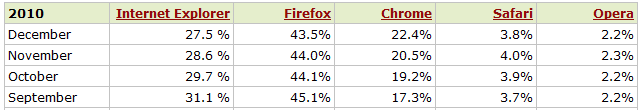
\includegraphics[width=.55\textwidth]{img/browser_statistics.png}
\caption{Market Share of Web Browser}
\label{figure:Market Share of Web Browser}
\end{figure}
And as a web development company, that is even less of an option. (your clients won't like that if you tell them that only 30 of the internet users will be able to use their website.)
Web application that behaves the same way in multiple browser are called "cross-browser". 
My job was of course to make sure that every web content I created was cross-browser (at least for IE7, IE8, Chrome and FF).
At first, this can look like a hard task to accomplish, because you would need to be aware of each browser specificities. Fortunately, some tools exists to help you reach that goal.

\subsubsection{JavaScript}

JavaScript has some big differences between browsers. For example, to attach an event to an element, Firefox and Chrome uses the function addEventListener. Internet Explorer will not understand this function as it uses attachEvent for the same purpose. %(cf Appendix page ## http://www.quirksmode.org/dom/w3c\_CSS.html).
Also, one of the purpose of JavaScript is being able to handle all the html elements in the web page to increase the user experience on the website. And again, there are some slight differences between every browser.
Because of all those disparities, people started to build APIs, which would considerably reduce the knowledge needed of those disparities to run a cross-browser JavaScript code. On of the most famous is jQuery. Simple, yet powerful, you can find in jQuery all the JavaScript functionalities, encapsulated in cross-browser functions. Ex: instead of having to test if the browser is IE to call the function attachEvent instead of addEventListener, you can just call the jQuery method bind to attach an event to an element. No need to learn the supported functions of each browser, you just need to learn a simple API. jQuery even simplifies some JavaScript functionalities, such as the use of Ajax.
%(cf piece of code w w/o jQuery).

\subsubsection{CSS}

Unlike in JavaScript, there is no API to help you with CSS (mainly because CSS is not a programming language). The huge issues in CSS arises when you want to make it work on Internet explorer. Usually, you are going to develop with Chrome or Firefox (Internet Explorer can be very slow so it can be frustrating to develop on it) where the same CSS is going to work on each other. It might even work in Internet Explorer 8 (with some really little adjustment on precise cases). But most of the time, you are going to have to do some adjustments so that it works on Internet Explorer 7. Those adjustment might be to just rethink the way of styling an element so that the same CSS will work on IE7 or completely tweaking the CSS just for Internet Explorer.
The last is called "CSS hacking". And fortunately, probably because Microsoft knows that his CSS handling is not that good, it introduced what is called conditional comments. It looks like a simple html comments in the html content, but IE knows it is aimed at him and can process it to add a specific Stylesheet. Other browsers will just ignore it, as it is a mere comment for them. (cg example html + speak about prefix * \_ etc.). 
\begin{figure}[!r]
\centering
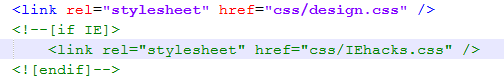
\includegraphics[width=.55\textwidth]{img/comments.png}
\caption{Conditional Comment}
\label{figure:conditional comment}
\end{figure}
Another way to tweak the CSS specifically for Internet Explorer is to add a specific prefix to each CSS property you want to be applied only to some Internet Explorer Versions. (prefix * : IE 7 and below,prefix \_: IE6 and below). The downside of this is that it renders the CSS invalid to the W3C specification.

Understanding all that, you can understand why creating a site builder application is even more of a challenge. Indeed, we have to provide the user that has no understanding of html, CSS or JavaScript the ability to create a cross-browser website. And that was an important point, because it could give us an advantage against other competitors, who are not always cross-browser compliant.




\chapter{Productivity tools}
As we we began the development of the Easy Web Content Site Builder from scratch, it gave us the opportunity to set-up a bunch of productivity tools. These tools are about automatize tasks, enhance code quality, debug, teamwork, documentation.

None of the following tools were implemented before I arrived in Hindsite Interactive. 
\section{Pear}

PEAR is a framework and distribution system for reusable PHP components. It allows to easily install, remove and update PHP libraries and packages by using simple command line.

\lstset{language=bash}
\begin{lstlisting}[label=pear-install,caption=Installation of pear packages]
C:\...>pear channel-discover channelname
C:\...>pear install --alldeps channelname/packagename
\end{lstlisting}

\section{Phing}

To work more efficiently, we implemented automatic build task tools . Phing is a build tool written in PHP. It is very similar to the famous ANT. Phing build tasks have been set to automatize js/css minification with the YUI Compress tool.
Right now we can use it to automate deployment and development.
\begin{itemize}
\item automatic js / css minify for release
\item automatic backup
\item automatic database deployment
\item generate php documentaion from comments
\end{itemize}

Phing uses pear to be installed automatically.

\lstset{language=bash}
\begin{lstlisting}[label=phing-install,caption=Installation of Phing]
C:\...>pear channel-discover channelname
C:\...>pear install --alldeps channelname/packagename
\end{lstlisting}

The build is configured with an xml file : build.xml. It allows to program automated tasks called targets. Targets can be combined and ordered.
Obfuscate JavaScript or CSS file would have been a very repetitive and boring task to do manually. This tool allows to keep the code non obfuscated for development environment (easy to debug and read), and obfuscated in production environment (lighter, faster and harder to read).

\lstset{language=Ant}
\begin{lstlisting}[label=phing-build,caption=Example of Phing build.xml]
<project name="EasyWebSite" basedir="." default="info">
	<property name="ProjectVersion" value="0.0.1" />
	<target name="minify-js">
		<minify targetDir="${releaseDirectory}/Framework/public/js/"
				yuiPath="${buildScriptsDirectory}/yuicompressor-2.4.2.jar">
			<fileset dir="${applicationDirectory}/Framework/public/js/">
			<include name="**/*.js"/>
			<exclude name="library/**"/>
			</fileset>
		</minify>
	</target>	
	<target name="zip-backup"
		description="Creates a backup of the project">
		<echo msg="Backup to zip archive"/>
		<copy file="build.xml" tofile="build.xml.backup" overwrite="true"/>
		<mkdir dir="${backupDirectory}" />				
		<zip destfile="${backupDirectory}/ews_backup-${ProjectDate}.zip">
		<fileset dir=".">
			<include name="build.xml" />
			<exclude name="build/**"/>
			<exclude name="docs/**"/>
			<include name="src/**" />			
		</fileset>
		</zip>
	</target>
	<target name="build-all" depends="cleanup , setup-environments, prepare-libs , execute-phpdoc, execute-jsdoc , deploying-debug, deploying-release, minify-js ,minify-css, deploy-database"
		description="deploys full environment">       
		<echo msg="Fin du build" />		
	</target>		
</project>
\end{lstlisting}

\section{Subversion}

Subversion is a version control system. It allows to keep track on modifications of files revision after revision. A system like this is very important to use in a team environment. For several reasons.

\paragraph*{Critic portions of code}
When working on important pieces of code the developer is often afraid to introduce bugs or to make the application crash. With a version control system, he can roll-back to previous stable versions of the code easily. So he can experiment new features with more confidence. 

\paragraph*{Debug}
If a bug is introduced, the developer can check what were the modifications in which files by using a 'diff' tool to compare two revisions of a the same file.

\begin{figure}[!ht]
\centering
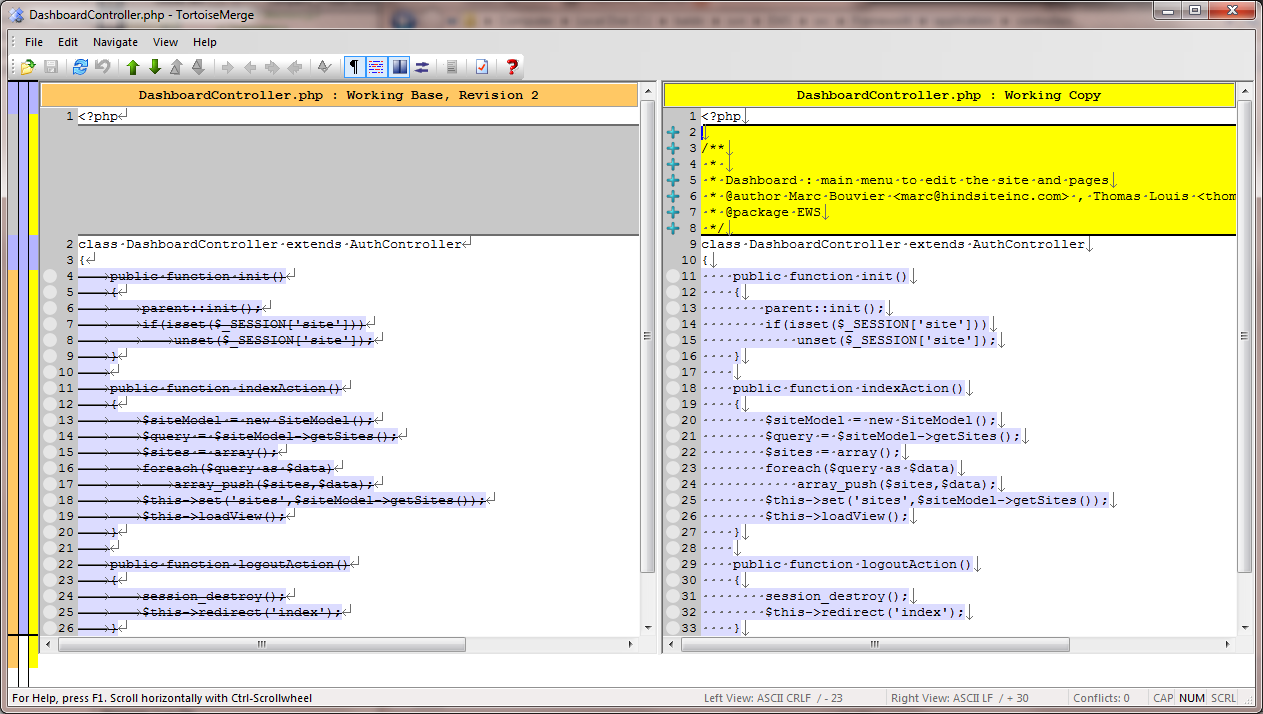
\includegraphics[width=.85\textwidth]{img/diff.png}
\caption{Diff tool}
\label{figure:diff}
\end{figure}

\paragraph*{Team-work}
When working in on a project with several developers, it is very important to work on the same versions of the project's file. Subversion stores the project in a repository from where the developers download incrementally the latest modifications of the files. So, only new or modified files are updated. Two developers may work on the same file at the same time because Subversion possess file merge and conflict resolution capabilities. It avoids overwriting a file that another developer would have modified.

\section{Code documentation}
Our applications and precisely the Site Builder project need to be maintenable and scalable. 

When I arrived at Hindsite Interactive and began working on the Easy Web Content project, I had to read a lot of documentation about the architecture of different components, but there was no document of the actual functions in the code. To understand the code and be able to debug it, having code documentation is a must.
\subsection{PHPDoc}
PhpDoc is a PHP framework that allows to generate web documentation of a project by using comments in the PHP code.

\begin{figure}[!ht]
\centering
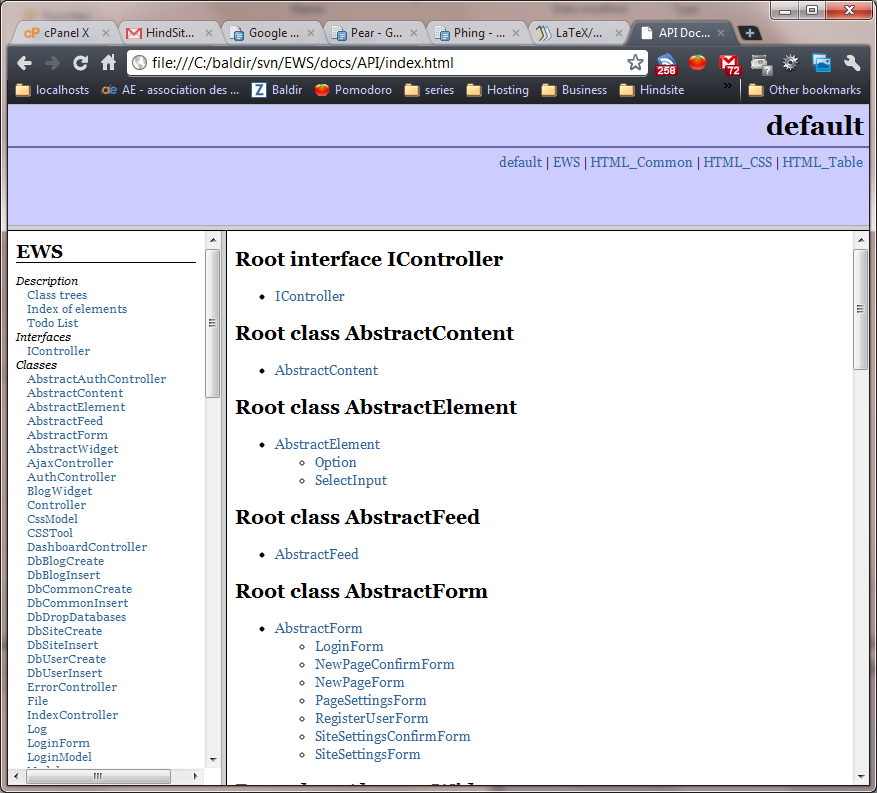
\includegraphics[width=.55\textwidth]{img/phpdoc.png}
\caption{Generated PHP Documentation from PHP code}
\label{figure:phpdoc-web}
\end{figure}

\lstset{language=PHP}
\begin{lstlisting}[label=phpdoc-code,caption=PHP documentation in a PHP class]

/**
 * 
 * Controller. 
 * The controller receives input and initiates a response by making calls on model objects.
 * A controller accepts input from the user and instructs the model and viewport to perform
 * actions based on that input.
 * @author Marc Bouvier <marc@hindsiteinc.com> , Thomas Louis <thomas@hindsiteinc.com>
 * @package	EWS
 */
class Controller implements IController{
	
	/**
	*	Boolean remains to false if no error occured, else set to true
	*	@var boolean
	*/
	protected static $error = false;

	/**
	 * 
	 * Constructor for the class Controller
	 * @param unknown_type $controllerName
	 * @param unknown_type $action
	 */
	public function __construct($controllerName, $action, $queryString=array()) 		{
		//some code
	}
\end{lstlisting}


\subsection{JSDoc}
JsDoc is a Javascript framework that allows to generate web documentation of a project by using comments in the Javascript code.

\begin{figure}[!ht]
\centering
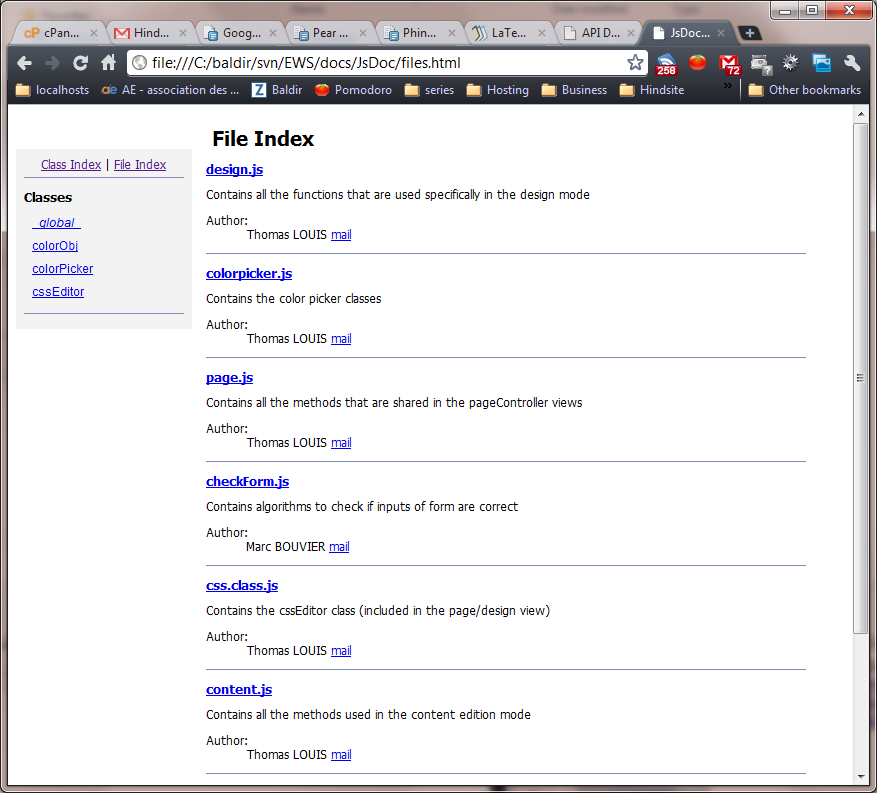
\includegraphics[width=.55\textwidth]{img/jsdoc.png}
\caption{Generated Javascript Documentation from Javascript code}
\label{figure:jsdoc-web}
\end{figure}

\lstset{language=Javascript}
\begin{lstlisting}[label=jsdoc-code,caption=Javascript documentation in a Javascript class]
/**
*	@fileOverview Contains the cssEditor class (included in the page/design view)
*	@author Thomas LOUIS <a href="mailto:thomas@hindsiteinc.com">mail</a>
*/

/**
*	@class Base class to set the css string and elements that the user wants to modify
*	@author Thomas LOUIS <a href="mailto:thomas@hindsiteinc.com">mail</a>
*/
cssEditor = function(target)
{
	/**
	*	Target of the click (it is a jQuery Object)
	*	@type Object
	*/
	this.target = target;

/**
*	Sets the inline property so that the user can see right away the changes applied to his page
*	@param {String} cssProperty The css property to be applied
*	@param {String} cssValue The property value
*	@todo Look and change the function
*/
cssEditor.prototype.setCss = function(cssProperty,cssValue)
{
	// some code		
}

\end{lstlisting}

\section{Netbeans}

Since we used Object Oriented Programming with PHP we had more needs of tools 
to write the code. Especially an IDE \footnote{Integrated Development Environment}.

\begin{itemize}
\item code autocompletion
\item code navigation
\item code syntax recognition
\item classes heritage detection
\end{itemize}


\section{Mantis}
Hindsite Interactive uses a lot Google documents to track tasks and issues. This allows to work on the same documents with other people of the team. The problem of this system is that it is not very efficient to manage tasks and bugs. It is like you track bugs in a Word document.

We have set up a bug tracker for internal use called Mantis it allows fast bug reporting. It allows Prioritization, importance management ... and assignment of issues to resolve. This allows everyone to keep track of the specific tasks they need to accomplish, and the bugs they need to resolve.


\begin{figure}[!ht]
\centering
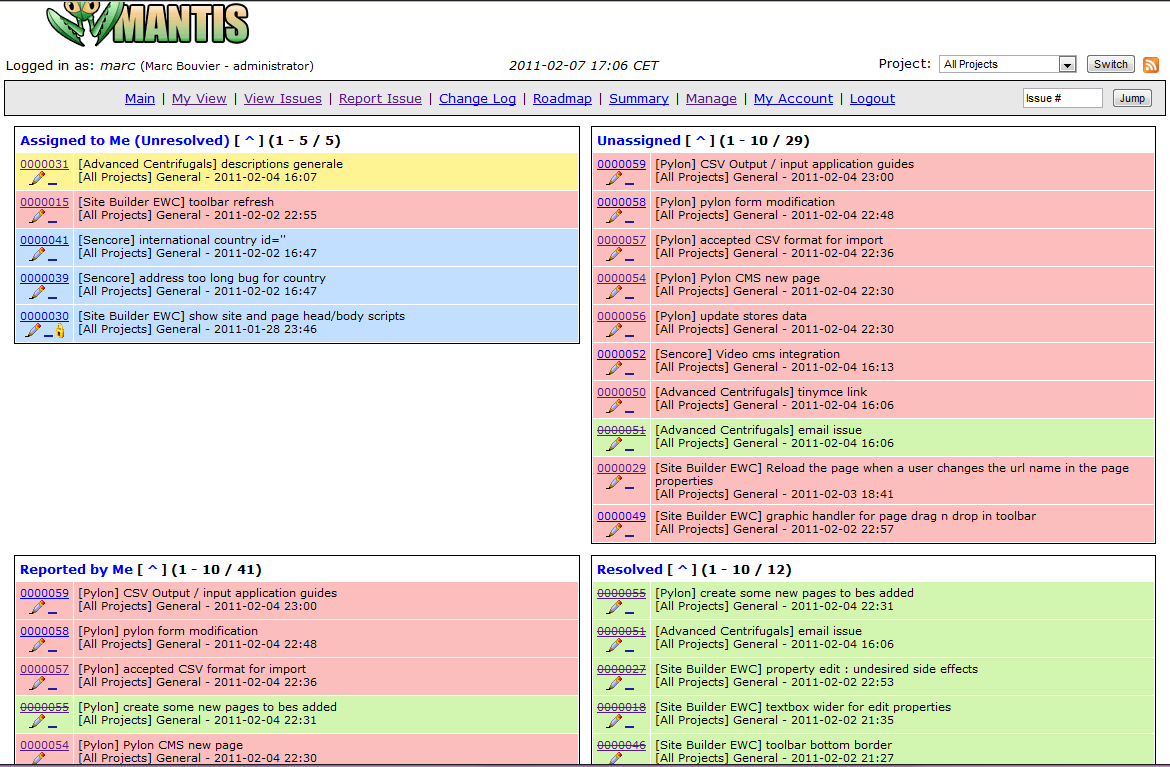
\includegraphics[width=.85\textwidth]{img/mantis.png}
\caption{Mantis tasks and issues multi-project view}
\label{figure:mantis}
\end{figure}
 


\chapter{Clients projects}


\chapter{Conclusion}

\section*{Overview of the work achieved}

%During this internship I completed the realization of three add-ons (Flash Maker,
%Calendar and Carousel) as well as an administrator for current and further HTML
%add-ons.
%These add-ons were tested and approved by my tutor but in my opinion we need to
%take more time to test all configuration cases, especially since there are so many
%cases that we cannot reproduce.
%
%One thing that definitely remains to do is add more templates, more presets to these
%add-ons to provide to the user a lot more possibilities of customization and
%examples. This part concerns more the designers that need to imagine and create
%templates and a small intervention from developer to integrate these.
%
%We are also expecting to launch last version of Easy Web Content containing all new
%add-ons soon so we can have feedback from users.
%
%We also have a lot of ideas for new add-ons that should be easier to create since we
%now have all required bases.
%
%I am now staying at Hindsite six other months to go on with this project, form next
%interns to this system and manage all further developments in this project.
%
%As Easy Web Content is not live at the moment I’m writing these lines we do not
%have an idea of the revenues generated through my work but I already know that
%when next version will be launched we will propose users two different subscriptions:
%- Standard account type will grant access to already existing functionalities of
%Easy Web
%- A new “Complete” account will give a full almost unlimited access to all add-
%ons to the user
%
%This Complete account will be proposed at a price of \$24.95 a month whereas
%standard account is at \$9.95.
%As the Complete account added value is important we hope to generate good
%revenues from this subscription and expect many users to switch to this account.

\section*{Work and organization}

%I feel like my work was really useful because I could see the results of it.
%In the United States the hours of work per week are greater than in France (around
%40 hours) and I was mostly satisfied with the progression of my work.
%I was granted a lot of independency in the choice of technologies, implementation,
%methods and organization. I could always give my opinion and submit my ideas.
%In the other hand I think that we can still improve a lot the organization of the work at
%Hindsite.
%
%For example we do not have any Subversion (CVS) to work with and as we were at
%least two people working on shared resources this was always a pain to work with
%and it happen that we lose time because of that.
%This is a point that me and previous interns already talked about to Mr. Taei but
%because do not have access to the server configuration we cannot configure a SVN
%ourselves.
%
%Another improvement of organization would be to use a Bug Tracker tool; we are still
%working with shared documents to track bugs.

% Pour finir l'interligne de 1,5
\end{onehalfspace}

%----------------------------------------
% Pour la bibliographie
%----------------------------------------
% Citer tous les ouvrages/références
% pour ajouter des references : ouvrir biblio.bib
%nocite permet d'ajouter de la biblio sans avoir aciter 
%quelquechose dans le document
\chapter*{Bibliography}

\subparagraph*{PHP}
\url{http://www.php.net/}

\subparagraph*{MySQL}
\url{http://dev.mysql.com/doc/refman/5.1/en/}

\subparagraph*{JQuery}
\url{http://jquery.com/}

\subparagraph*{Scriptaculous}
\url{http://script.aculo.us/}

\subparagraph*{PHPDoc}
\url{manual.phpdoc.org/ }

\subparagraph*{JSDoc}
\url{http://jsdoc.sourceforge.net/}

\subparagraph*{Pear}
\url{http://pear.php.net/}

\subparagraph*{Phing}
\url{http://phing.info/trac/}
\printindex
%exemples d'annexes
\appendix
\part*{Appendix}

\chapter{Site Builder Competitors}\label{annexe:ews-competitors}
\begin{figure}[!ht]
\centering
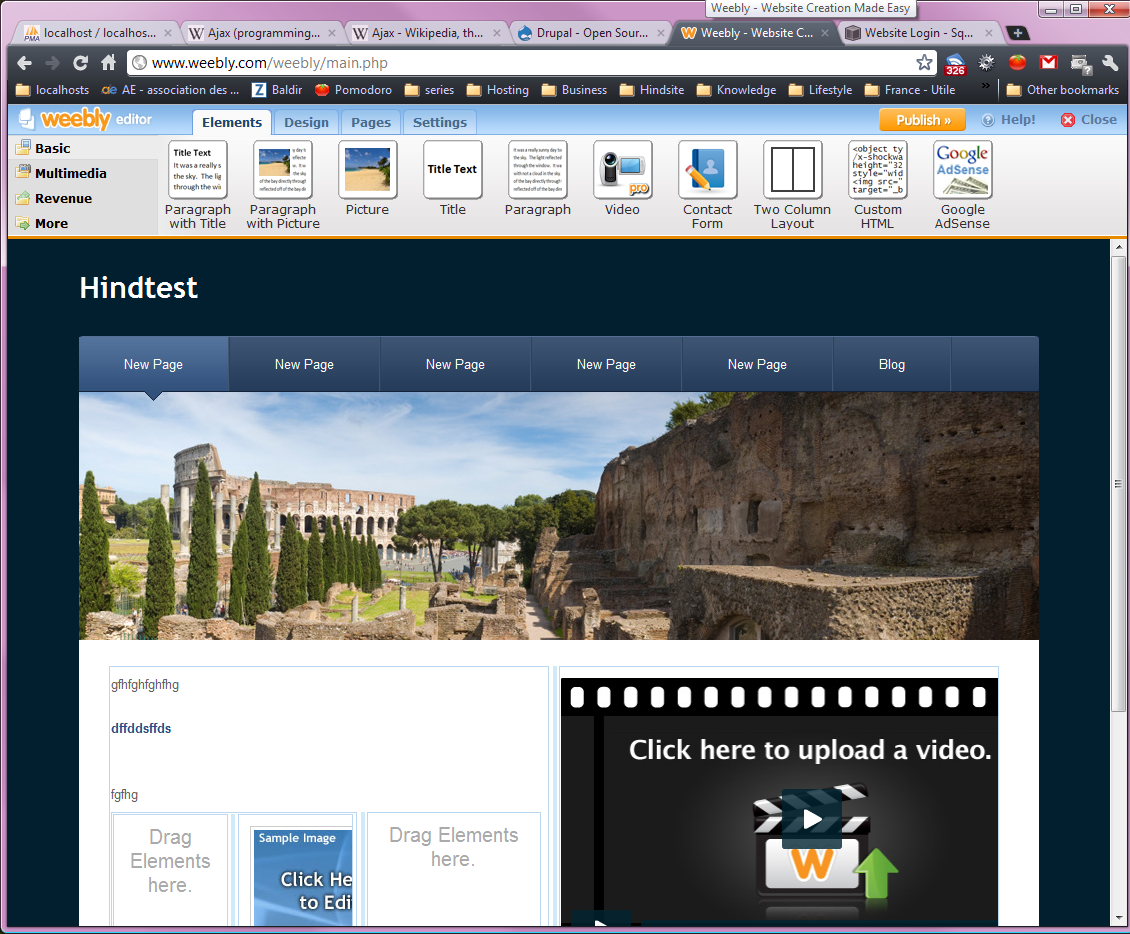
\includegraphics[width=.70\textwidth]{img/weebly.png}
\caption{Weebly}
\label{figure:weebly}
\end{figure}

\begin{figure}[!ht]
\centering
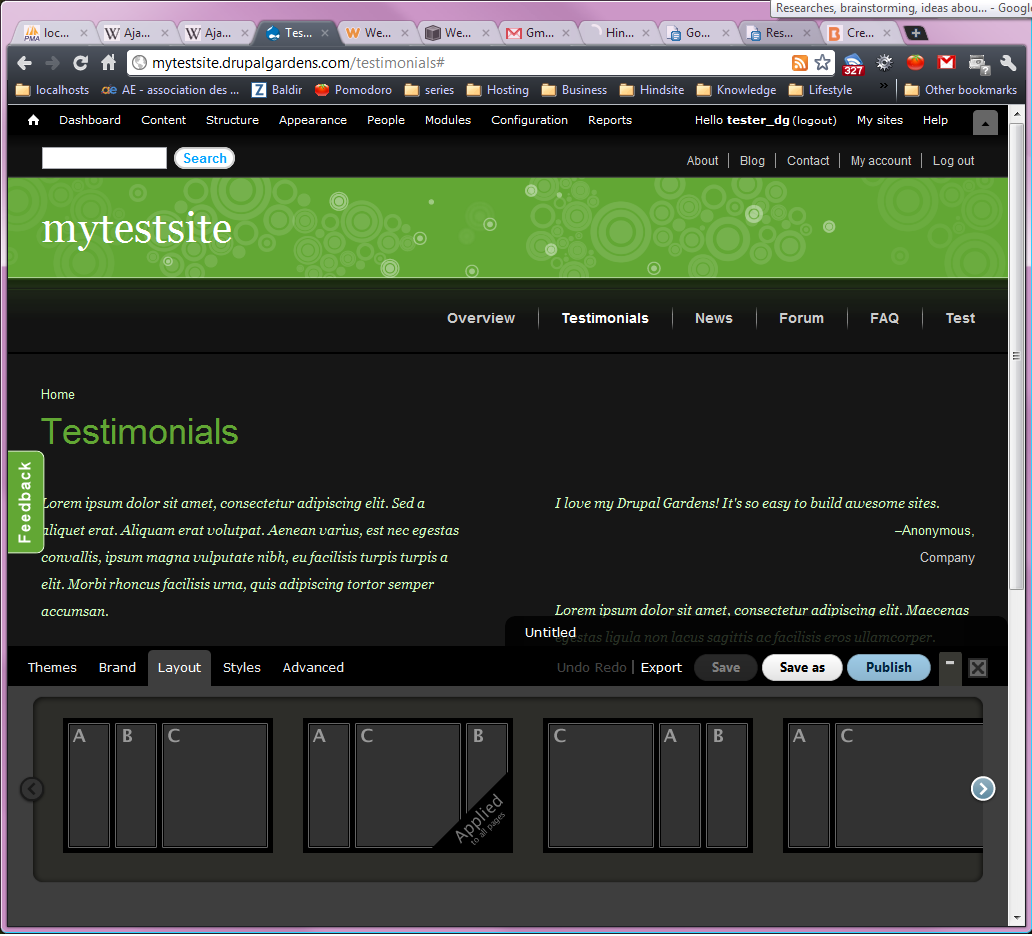
\includegraphics[width=.70\textwidth]{img/drupal_gardens.png}
\caption{Drupal Gardens}
\label{figure:drupal_gardens}
\end{figure}

\begin{figure}[!ht]
\centering
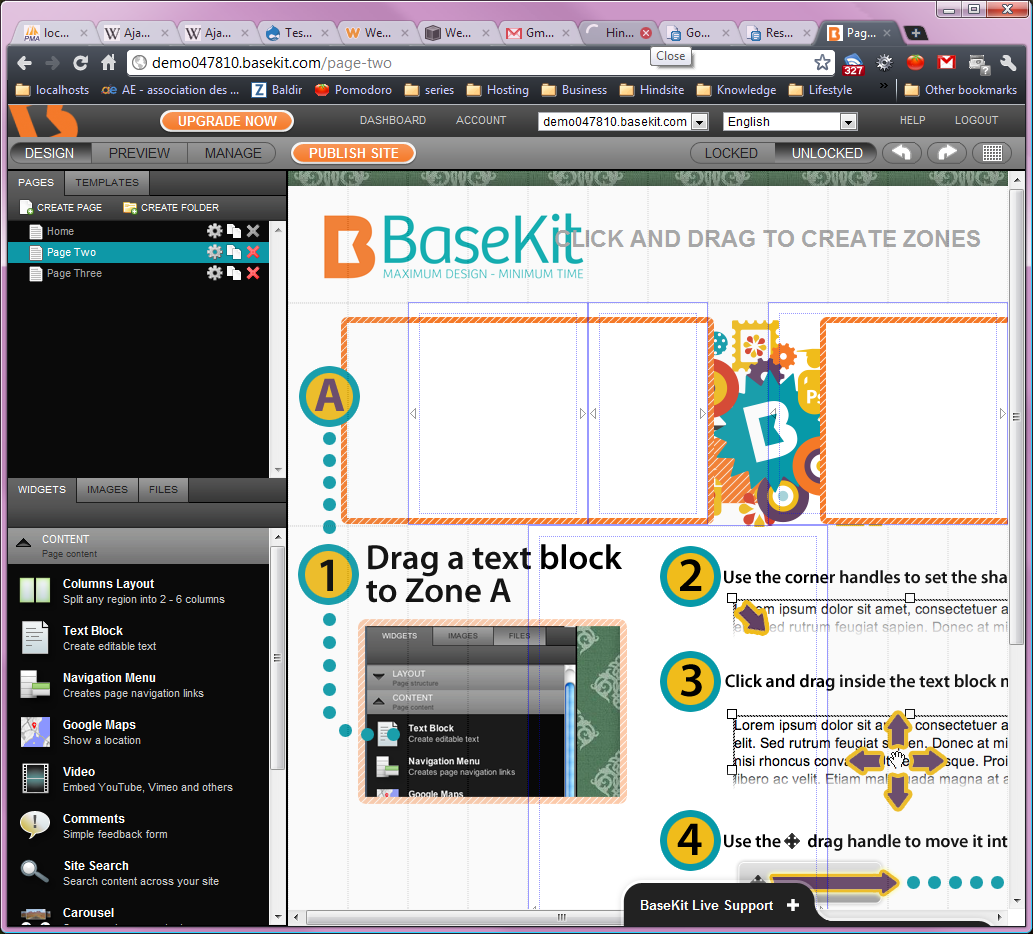
\includegraphics[width=.70\textwidth]{img/basekit.png}
\caption{BaseKit}
\label{figure:basekit}
\end{figure}

\begin{figure}[!ht]
\centering
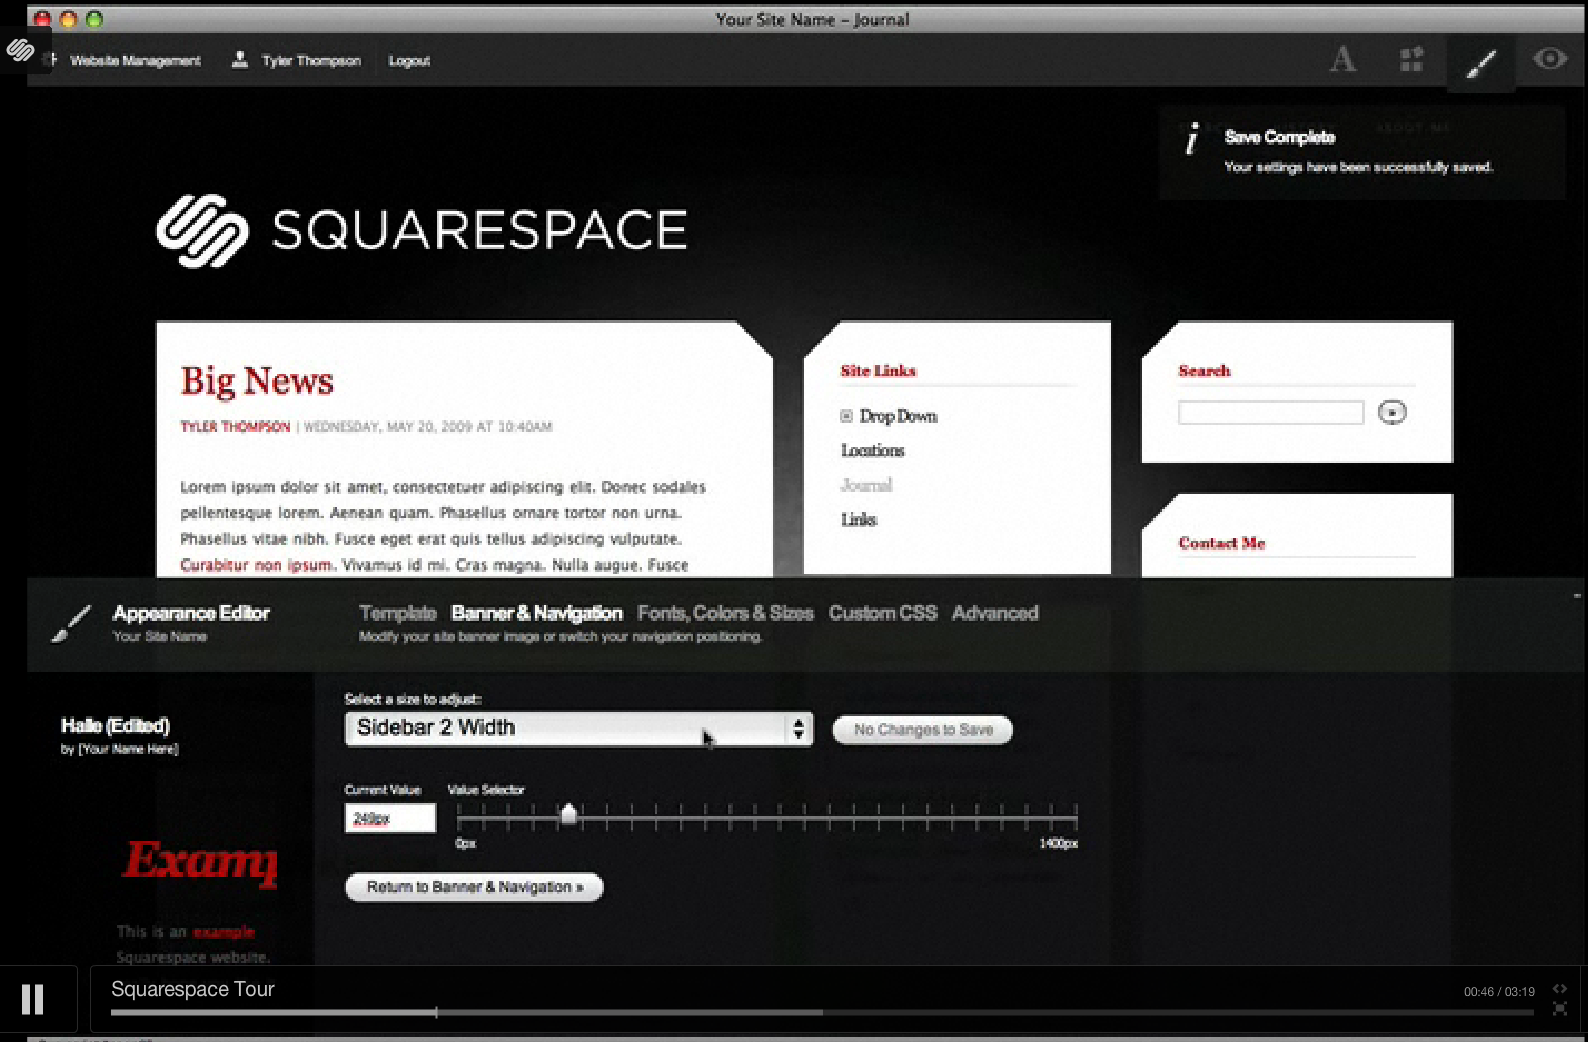
\includegraphics[width=.70\textwidth]{img/squarespace.png}
\caption{Squarespace}
\label{figure:squarespace}
\end{figure}
\chapter{Cross browser issues}\label{annexe:JavaScript differences}


\section*{Example of javascript differences between browsers}
\begin{figure}[!ht]
\centering
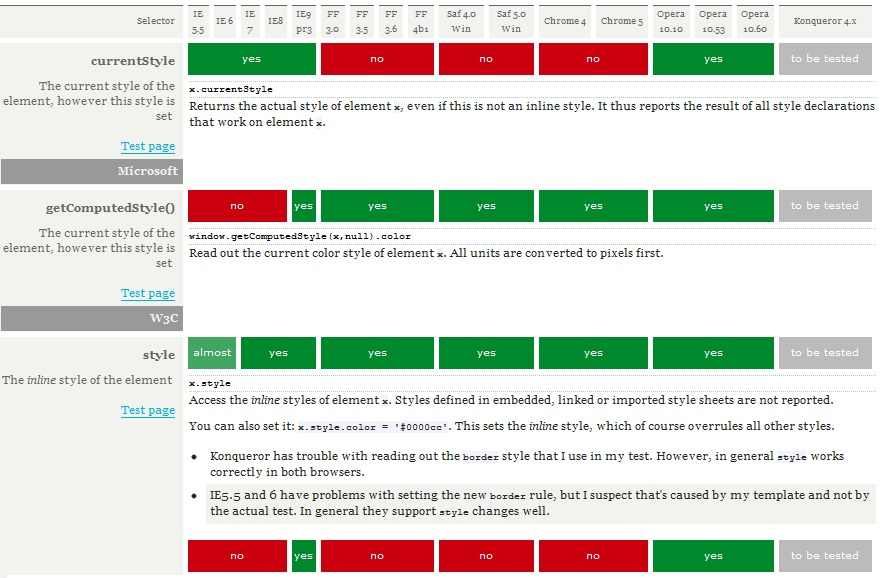
\includegraphics[width=\textwidth]{img/css.jpg}
\caption{Css handling differences}
\label{figure:market-brosers}
\end{figure}


%\chapter{Pomodoro Technique}\label{annexe:pomodoro}

\paragraph*{Qu'est ce que c'est?}La technique du pomodoro a été inventée par Fransesco Cirillo. C'est une technique de gestion du temps qui peut être utilisée pour n'importe quelle type de tâche. L'objectif de la technique du pomodoro est de considérer le temps comme un allié dans ce que l'on veut faire et d'améliorer en permanence notre façon de travailler ou d'étudier.

\paragraph*{Que faut-il pour commencer?}
\subparagraph*{Une minuterie de cuisine}
Vous pouvez aussi bien utiliser un pomodoro\footnote{minuterie de cuisine} qu'un timer logiciel. Le régler sur 25 minutes.

\clearpage
% 4eme de couverture

\includepdf[pages=1,noautoscale=false]{Couv_rapportverso_Marc.pdf}
\end{document}
